%!TEX root = ../dissertation.tex

\chapter{Model and approach}
\label{ch:model}

\section{Model}

In the following sections we describe the model architecture, outlined
in Fig.\ref{fig:model-architecture}. We first delineate the visual and
textual branch in Sec.~\ref{subsec:visual-branch} and
\ref{subsec:textual-branch}. We then present the concept similarity,
our novel contribution, in Sec.~\ref{subsec:similarity-branch}, along
with the prediction and loss modules in
Sec.~\ref{subsec:prediction-module} and \ref{sec:loss}. We then
conclude highlighting the training and inference protocol in
Sec.~\ref{sec:training-and-inference}.

\begin{figure}
  \centering
  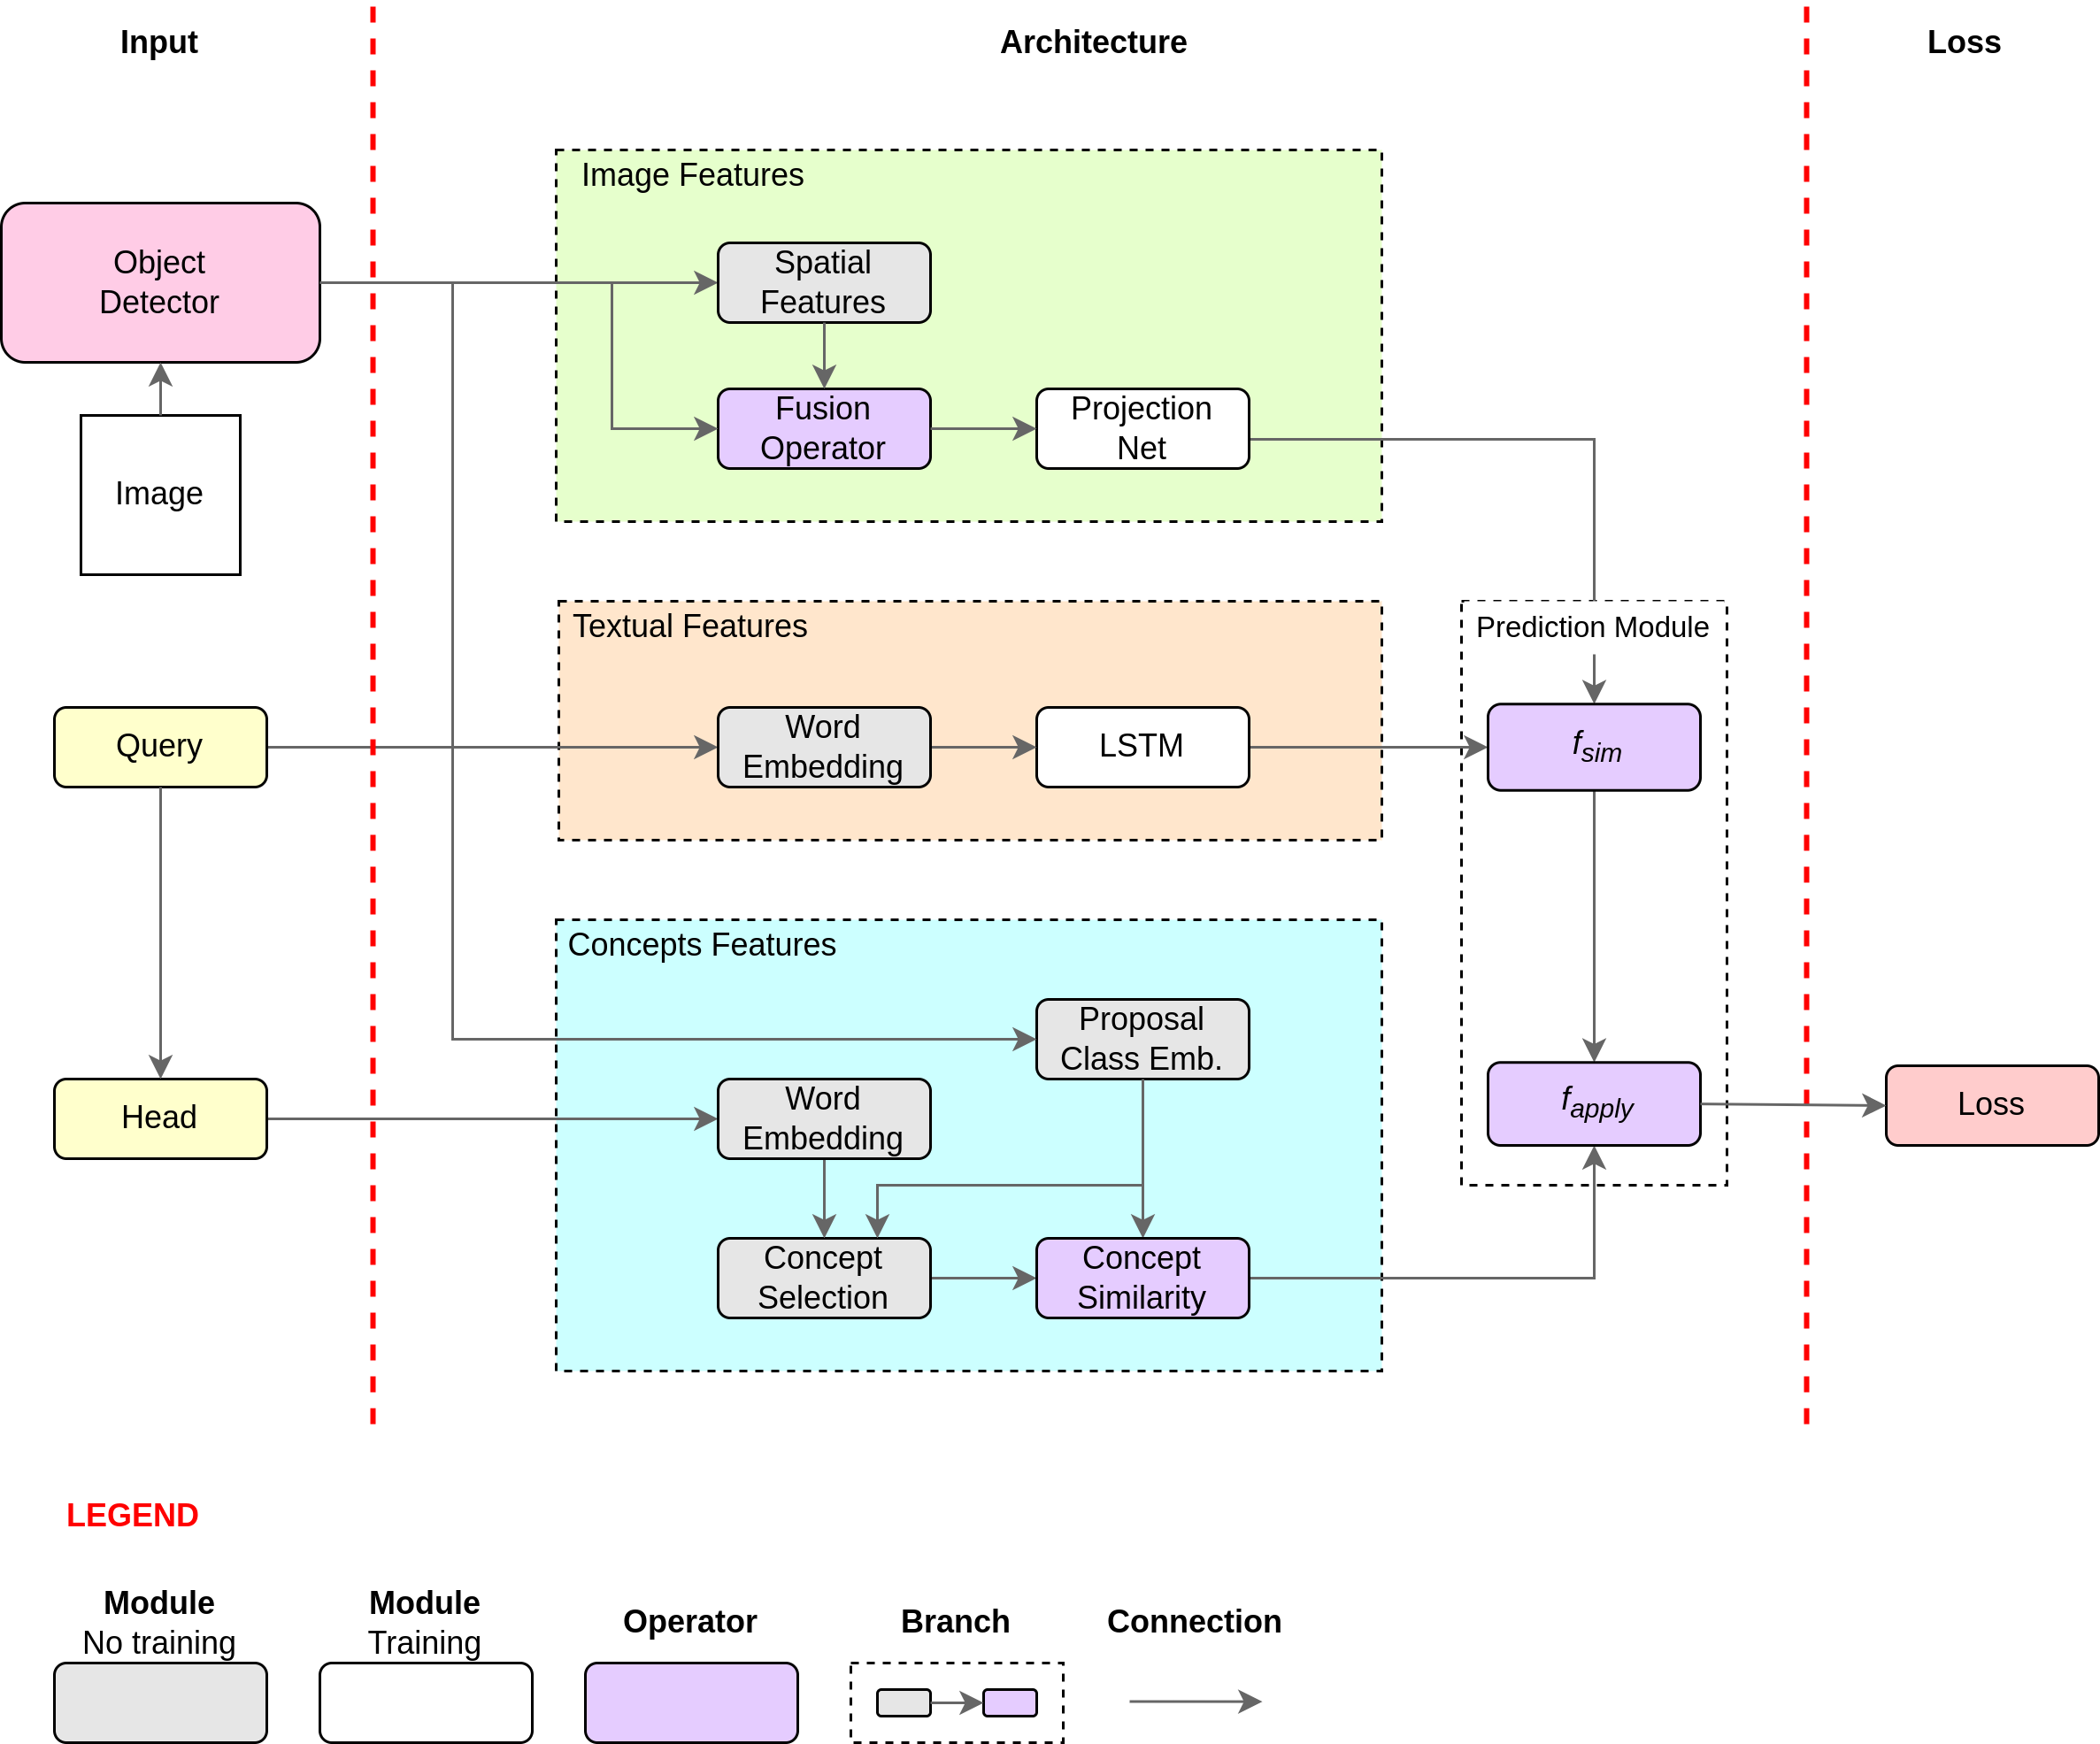
\includegraphics[width=1.0\textwidth]{figures/model-architecture.png}
  \caption[Model architecture overview]{ Our model architecture
    overview. Initially, the image is processed by a pre-trained
    Faster R-CNN object detector in order to extract all the proposals
    bounding boxes from which the spatial features are generated.
    Then, the model generates textual features from the input noun
    phrase by first retrieving each word embedding and then using an
    LSTM network. Finally, the model fuses together all the visual,
    spatial, and textual features by the Fusion Operator. Those
    features are then used by the model in combination with textual
    feature to predict a score of similarity between the two. The
    concept branch predict another similarity score between the word
    embedding of concept the phrase and the class label on proposal.
    Such score is applied to models predictions as a prior and fed
    into the loss module that optimizes positive scores to be larger
    than negative scores. }
  \label{fig:model-architecture}
\end{figure}

\subsection{Visual Branch}
\label{subsec:visual-branch}

Given an image $\bm{I}$, we extract a set of $k$ bounding box
proposals $\calP_{\bm{I}} = \{ \bm{p}_z \}^k_{z=1}$ by means of a
pre-trained object detector where $\bm{p}_z \in \Rset^4$, jointly with
features $H^v = \{ \bm{h}^v_z \}^k_{z=1}$, where $\bm{h}^v_z \in
\Rset^v$. The features represent the internal object detector
activation values before the classification layers and regression
layer for bounding boxes. Moreover, our model extracts the spatial
features $H^s = \{ \bm{h}^s_z \}^k_{z=1}$, where $\bm{h}^s_z \in
\Rset^s$ from all the bounding boxes proposals, with the spatial
features for the proposal $\bm{p}_z$ defined as:
\begin{equation}
  \bm{h}^s_z = \left[ \frac{x1}{wt}, \frac{y1}{ht}, \frac{x2}{wt}, \frac{y2}{ht}, \frac{(x2 - x1) \times (y2 - y1)}{wt \times ht}  \right]
\end{equation}
where $(x1, y1)$ refers to the top-left bounding box corner, $(x2,
y2)$ refers to the bottom-right bounding box corner, $wt$ and $ht$ are
the width and height of the image, respectively. At this point, for
each $\bm{p}_z \in \calP_{\bm{I}}$ we are given $\bm{h}^v_z$ the
object detector internal activation features and $\bm{h}^s_z$ the
spacial features that encode proposal coordinates in the image. We
also assume that the object detector returns, for each $\bm{p}_i$, a
probability distribution $Pr_{Cls}(\bm{p}_i)$ over a set $Cls$ of
predefined classes, i.e. the probability for each class $\zeta \in
Cls$ that the content of the bounding box $\bm{p}_i$ belongs to
$\zeta$. This information is typically returned by most of the object
detectors, and it will be used in Sec.~\ref{subsec:similarity-branch}
to define the concept similarity.

Both visual and spatial features are then concatenated and projected,
thus leading to a set of new vectorial representations $H^{||} = \{
\bm{h}^{||}_{z} \}_{z \in [1, \ldots, k]}$, where vectors
$\bm{h}^{||}_{z}$ are defined as:
\begin{equation}
  \bm{h}^{||}_{z} = \bm{W}^{||} \big( \bm{h}^s_z || L1(\bm{h}^v_z) \big) + \bm{b}^{||},
  \label{eq:h-par-jz}
\end{equation}
where $||$ indicates the concatenation operator, $\bm{h}^{||}_{z} \in
\Rset^c$, $\bm{W}^{||} \in \Rset^{c \times (s + v)}$ is a matrix of
weights, $\bm{b}^{||} \in \Rset^c$ is a bias vector, and $L1$ is the
L$1$ normalization function.



\subsection{Textual Branch}
\label{subsec:textual-branch}

Regarding the textual features extraction, given a noun phrase
$\bm{q}_j$, initially all its words $W^{\bm{q}_j} = \{ w^{\bm{q}_j}_i
\}^l_{i=1}$ are embedded in a set of vectors $E^{\bm{q}_j} = \{ \eqj_i
\}^l_{i=1}$ where $\eqj_i \in \Rset^w$, where $w$ is the size of the
embedding. Then, our model applies a LSTM neural network
(Sec.~\ref{subsec:gated-rnn}) to generate from the sequence of word
embeddings only one new embedding $\bm{h}^*_j$ for each phrase
$\bm{q}_j$. This textual features extraction is defined as:
\begin{equation}
  \bm{h}^*_j = L1(LSTM(E^{\bm{q}_j}))
  \label{eq:h-star}
\end{equation}
where $\bm{h}^*_j \in \Rset^t$ is the LSTM output of the last word in
the noun phrase $\bm{q}_j$, and $L1$ is the L$1$ normalization
function.

\subsection{Similarity Branch}
\label{subsec:similarity-branch}

Along with visual and textual features we also compute a similarity
score between noun phrases and bounding boxes: the concept similarity
\cite{wang2019phrase}. The aim of such score is to capture the
semantic similarity between the content of a proposal and the concept
expressed by a phrase. But, instead of learning a complex multimodal
mapping function between features, which is very difficult to realize
in weakly supervised settings, we directly combine information given
by object detector and phrases. More precisely, we exploit those
information by leveraging on pretrained word embeddings. A good set of
word embeddings is able to capture, above all, the semantic similarity
between words, hence, words with same meaning should have similar
representation (Sec.~\ref{sec:word-embeddings}). Based on this
assumption, the similarity score can be trivially expressed as a
distance measure between two vectors in a space. Thus, we define the
concept similarity as a distance measure between to two word
embeddings, i.e., concepts. The word embedding that express proposal
concept is extracted from predicted proposal class, usually returned
from object detector as a probability distribution over a set of
labels (Sec.~\ref{subsec:visual-branch}). We can easily gather the
label that best express proposal's content by simply taking the label
with maximum probability. Such label is just a word (or, in few cases
a combination of words), that can be naturally embedded in the word
embeddings space. However, we noticed many misspells and confusion
among class labels. For example, some labels are made by more than one
word (``christmas tree'', ``rock wall''), while some other contains
many different versions of the same word (``microwave, microwave
oven'', ``tennis racket, tennis racquet''). Thus, following
\cite{wang2019phrase} we fix misspells by an external spell correction
system,\footnote{\href{https://pypi.org/project/pyspellchecker/}{https://pypi.org/project/pyspellchecker/}}
while for compound and multi-version words, we first split them by
punctuation (space, column and dot) and we average over single-word
embeddings. Instead, the word embedding that express phrase concept
can be a single word or a combination of words from the phrase.
Following a similar idea of \cite{javed2018learning} where they
perform concept selection filtering out non-noun words, we select the
concept among heads of phrase. Heads are extracted trough an
off-the-shelf english language parser (Sec.~\ref{subsec:nlp-tools}). 

Formally, we define $\EPI = \{ \ePI_i \}^{k}_{i=1}$ where $\ePI_i \in
\Rset^w$ the set of labels embeddings build on the set of proposal
$\calP^{\bm{I}}$. Each $\ePI_i$ is a feature vector representing the
label predicted with maximum probability by the object detector for
the $i$-th proposal. Then, given a noun phrase $\bm{q}_j$ along with
$E^{\bm{q}_j}$, we compute the concept similarity score for each
proposal $\bm{p}_i$ as:
\begin{equation}
  \bm{S}^c_{ji} = \fsim \left( \erqj_j, \ePI_i \right),
\end{equation}
where $\fsim$ is a similarity measure (such us the cosine similarity),
and $\erqj_j$ is the embedding representing the concept of the noun
phrase $\qj$. The new embedding $\erqj_j$ can be computed with various
strategies, and we can group these into two main categories. The first
is the group where we can find operators that take into account the
entire phrase to generate a representative. A widely used strategy is
to generate a new embedding by averaging phrase's word embeddings:
\begin{equation}
  \erqj_j = \frac{\sum^l_{i=1} \eqj_i}{| \Eqj |},
\end{equation}
however, there is an evidence that such averaging operations can
compromise the discriminativeness
\cite{wang2019phrase,datta2019align2ground}. Averaging over all words
means to implicitly consider even irrelevant words for grounding,
which, on average, may impact on the representation of the concept.
This problem is partially reduced by model which extracts concept on
phrase by considering only phrase's head.

In the second group we find operators that consider a single word as a
representative for the phrase. A common strategy employed in
literature is to select the last word in the phrase
\cite{wang2019phrase}. Specially in English language, the last word of
a noun phrase is usually the head of the phrase. However, this
strategy relies on strong assumptions on language and how dataset is
built.\footnote{In \cite{wang2019phrase}, they show how the
\textit{last} strategy differs in performance on different dataset: on
Flickr30k Entities it is the second best strategy while in ReferIt it
doesn't even appear on the leaderboard.} More complex strategies,
instead, take into account additional information, such us the
similarity wrt proposal class embeddings. Here, a possible strategy
consists in choosing the phrase representative as the word with
maximum similarity wrt detected concepts among proposals. Following
\cite{wang2019phrase}, we compute the similarity between all words in
noun phrase and proposal class embeddings, and then we select one word
in the noun phrase with maximum similarity wrt the detected concept in
proposal:
\begin{equation}
  \erqj_j = \argmax_{\eqj \in \Eqj} \{ \max g(\eqj) \},
  \label{eq:concept-embedding-max-sim}
\end{equation}
where
\begin{equation}
  g(\eqj) = \{ \fsim(\ePI, \eqj) \mid \ePI \in \EPI \}.
\end{equation}
This strategy is better explained by means of an example, such us the
one in Fig.~\ref{fig:concept-selection-example}. For the sake of
presentation, we assume to deal with an object detector trained on two
class labels $Cls = \{ \text{sky}, \text{animal} \}$. We are given an
image (in figure) and the query ``the blue elephant''. As described in
Eq.~\ref{eq:concept-embedding-max-sim}, our model computes all
similarities between the embedding of words in phrase $\eqj$ and the
embedding of proposal's class labels $\ePI$. The representative
concept for the query is defined as the embedding of the word with
maximum similarity wrt proposals. In our example, the word
``elephant'' has maximum similarity with the proposal labeled with
\textit{animal}, so it becomes the concept of the phrase. Scores
associated with this concept will be used at prediction stage
(Sec.~\ref{subsec:prediction-module}) to downweight unrelated
proposals.

\begin{figure}
  \centering
  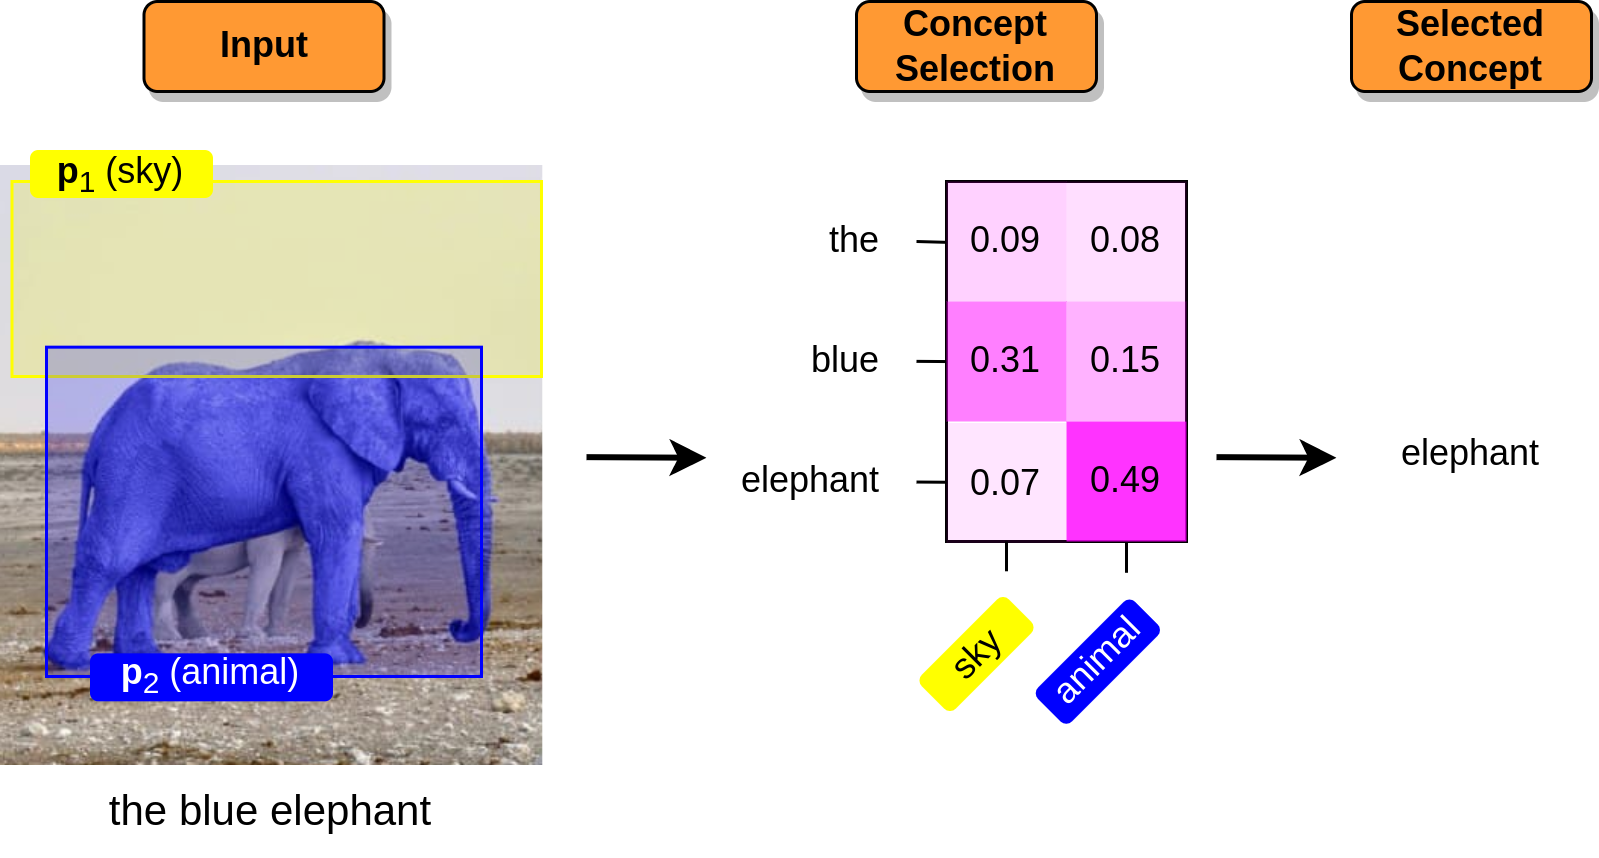
\includegraphics[width=0.8\textwidth]{figures/concept-selection-example.png}
  \caption[Concept selection example]{ TODO }
  \label{fig:concept-selection-example}
\end{figure}

\subsection{Prediction Module}
\label{subsec:prediction-module}

Finally, the model predicts the probability $\bm{P}_{jz}$ that a given
noun phrase $\qj$ is referrred to a proposal bounding box $\bm{p}_z$
as:
\begin{equation}
  \bm{P}_{jz} = \fsim ( \bm{h}^{||}_{jz} , \bm{h}^*_j ),
\end{equation}
where $\fsim$ is a similarity measure and $\bm{h}^{||}_{jz}$,
$\bm{h}^*_j$ are features extracted by visual and textual branch,
respectively.

As noted in \cite{chen2018knowledge}, concept similarity is a direct
consequence of the intrinsic knwoledge convoyed by the object
detector. Such score can be useful to downweight unrelated proposals.
Its effectiveness is due to the fact that the word embedding usually
captures the semantic similarity between concept in phrase and the
content of the bounding box, and thus, let the model focuses on
relevant proposals. Thus, a straightforward improvement to our base
model would be to include this knowledge and exploit it for making
predictions. Hence, predictions can be enhanced by multiplying the
two, treating $\bm{S}^c_{jz}$ as a weight matrix:
\begin{equation}
  \bm{\hat{P}}_{jz} = \bm{S}^c_{jz} * \bm{P}_{jz}.
\end{equation}
At first glance, this approach seems very promising because we force
the model to return predictions ``on steroid'' when there is a
semantic relation between phrase and proposal or downweighted when
little similarity is found. However, this relies on the assumption
that the embedding space and similarity measure we are using for words
perfectly captures the semantic similarity between them, and this is
not true. Also, we assume that proposals are classified with no error
by the object detector, neither this is true. Under those hypotesis,
such application of concept similarity cannot be fruitful. 

An example my clarify our statement. We are given $\bm{S}^c \in
\Rset^{1 \times 2}$, $\bm{S}^c = [0.1, 0.2]$ for an example composed by a
phrase and two proposal, and we know that the bounding box to ground
with our prhrase is the first. The only way the model has to output
the first proposal as the best bounding box, i.e., the bounding box to
ground, is to predict a score $p_{0}$ which is at least the double of
$p_{1}$, because
\begin{equation}
  \bm{\hat{P}} = [0.1 * p_{0}, 0.2 * p_{1}]
\end{equation}
and hence
\begin{equation}
\begin{split}
0.1 * p_{0} > 0.2 * p_{1} & \iff p_{0} >  \frac{0.2}{0.1} * p_{1} \\
  & \iff p_{0} > 2 * p_{1}.
\end{split}
\end{equation}
Here, $p_{j} = \bm{P}_{0,j}$. Thus, with such scores $\bm{S}^c$, when
the model predicts $0.1$ for $p_1$, it must learn to predict $> 0.2$
for $p_0$, when it predicts $0.5$ for $p_1$, it must learn to predict
$1.0$ (the maximum) for $p_0$ and when it predicts a value $> 0.5$ for
$p_1$ there is no way to predict a greater score for $p_0$. In
conclusion, the model isn't really able to learn and its completely at
the mercy of similarity scores.

A more convenient way of applying concept similarity to prediction is
instead to compute the mean between two. Eventually, we can also put a
weight $\lambda \in [0 .. 1]$ in order to balance
contributions. Formally:
\begin{equation}
  \bm{\hat{P}}_{jz} = (1 - \lambda) * \bm{S}^c_{jz} + \lambda * \bm{P}_{jz}.
\end{equation}
The major benefit of this approach is that model predictions are not
constrained to values defined by concept similarity: they co-work for
the final predictions.

\section{Loss Function}
\label{sec:loss}

In this section we present our loss function. Please note that in
weakly supervised settings, for a training example $\left( \bm{I}, S
\right)$ we are not given the query-proposal pair set $\{ ( q^{gt}_j,
p^{gt}_j ) \}^m_{j=1}$, where $m$ is the number of noun phrases.
Inspired by \cite{wang2020maf}, we adopt a contrastive loss. The
contrastive objective $\calL$ aims to learn the visual and textual
features by maximizing the similarity score between paired
image-caption elements and minimizing the score between the negative
samples (i.e., other irrelevant captions). Formally, given $\bm{I}$
the image, $S$ a sentence that describes $\bm{I}$ and $S'$ a sentence
that do not describe $\bm{I}$, we define $\calL$ as:
\begin{equation}
  \calL =  - \fmmsim(\bm{I}, S) + \fmmsim(\bm{I}, S'),
\end{equation}
where
$\fmmsim$ is the multimodal image-sentence similarity function, defined as:
\begin{equation}
  \fmmsim(\bm{I}, S) = \frac{1}{m} \sum_j \max_z \bm{P}_{jz}
\end{equation}
where $m$ is the number of noun phrases in $S$ and $\bm{P}_{jz}$ is
the predicted similarity between query $\bm{q}_j$ and proposal
$\bm{p}_z$. Basically, the goal of $\fmmsim$ is to express an averaged
representation of queries wrt the image.

In contrast of what done in \cite{wang2020maf} where they gather
negative sentences from batch, we randomly sample a single negative
sentence from the dataset.

\section{Training and Inference}
\label{sec:training-and-inference}

At training stage, we are given the example $(\bm{I}, S)$ where
$\calP_{\bm{I}} = \{ \bm{p}_i \}^k_{i=1}$ is the set of bounding box
proposals built on $\bm{I}$ and $\bm{q}_j$ are queries in $S$. As
noted in Sec.~\ref{subsec:visual-branch} we use extra information from
object detector such us the probability distribution on bounding box
class labels $Pr_{Cls}(\bm{p}_i)$. Following \cite{chen2018knowledge}
we fix $k = 100$ proposals. (We studied how $k$ can affect results in
Sec.~\ref{sec:data-analysis}). We optimize parameter of the LSTM
network (Eq.~\ref{eq:h-star}) and projection network
(Eq.~\ref{eq:h-par-jz}). We use the cosine similarity as similarity
measure $\fsim$ between vectors. Our network is trained end-to-end
using Adam optimizer with gradient clipping set to $1$ and learning
rate $0.001$.

At test stage, we feed the $\bm{q}_j$ and $\calP_{\bm{I}}$ to the
model. It predict a similarity score from $-1$ to $1$ for each
bounding box. The grounded proposal is defined as:
\begin{equation}
  \bm{p}_{z^*} \quad \text{s.t.} \quad z^* = \argmax_z \bm{P}_{jz}.
\end{equation}
According to \cite{wang2019phrase}, for some experiments we select the
grounded proposal as the union box of the proposal with the same class
label as the box predicted with maximum confidence $\bm{p}_{z^*}$:
\begin{equation}
  \bm{p}^u_{z^*} = \bigcup P_{z^*}
\end{equation}
where we intend $\bigcup$ on set of proposal as the union box
operator, $P_{z^*}$ is the set of proposal with same class label as
$\bm{p}_{z^*}$, thus:
\begin{equation}
  P_{z^*} = \{ \bm{p} \mid \bm{p} \in \calP_{\bm{I}} \land cls(\bm{p}) = cls(\bm{p}_{z^*}) \},
\end{equation}
where $cls(\bm{p}) = Cls_{\argmax_z Pr_{Cls}(\bm{p})}$ is the function
that returns the class label of a proposal.
